\section*{Market outlook}\label{sec:outlook}

Our reading of the macro picture is that 2026 has been a year of
stagflation, that economists expect a return to goldilocks in 2027, and
that markets do not share this optimism. Fed funds futures, in fact,
price about 3.4 further hikes, reaching roughly 100 basis points above
what economists forecast. Hence, we do not build the portfolio around a
single regime, but hold assets that perform in each of them.

\subsection*{Growth and inflation}\label{sec:growth-inflation}

We classify each economy into the four regimes defined by the direction
of growth and inflation, using the Bloomberg consensus forecasts. During
2026 inflation rose in every region, in the United States and in the
emerging economies it did so while growth was slowing: US CPI went from
2.7\% to 3.4\% and real GDP growth fell from 2.6\% to 1.8\%, which
places both economies in stagflation. For 2027, the consensus expects
growth to remain steady or to rise and inflation to fall in every
region, the pattern of a goldilocks economy (Table~\ref{tab:regimes}). \cite{ecfc}

\begin{table}[!htb]
\centering
\small
\caption{Consensus forecasts and macro regimes}\label{tab:regimes}
\begin{tabular}{@{}lrrrrl@{}}
\toprule
Region & GDP Q4 26 & GDP Q4 27 & CPI Q4 26 & CPI Q4 27 & Regime 2026 \\
\midrule
United States & 2.1\% & 2.1\% & 3.5\% & 2.1\% & Stagflation \\
Developed economies & 1.8\% & 1.9\% & 3.9\% & 2.5\% & Overheated \\
Emerging economies & 3.9\% & 4.4\% & 3.6\% & 2.9\% & Stagflation \\
\bottomrule
\end{tabular}

\smallskip
\footnotesize\emph{Real GDP and CPI, year-on-year. Regime 2026: direction of growth
and inflation from Q1 to Q3 2026. \cite{ecfc}}
\end{table}

Behind these numbers, the US economy is slowing gently rather than
contracting. Unemployment is stable at about 4.2\% and payroll growth
has eased to about 60,000 jobs a month, while private investment remains
the strongest component of demand, having grown at an annualised 7.4\%
in the third quarter. Inflation is still the main concern, with core PCE
at 3.3\%. Europe continues to grow slowly, at 1.3--1.6\%, whereas the
emerging economies combine rising growth with monetary easing, as their
central banks are expected to cut rates from 6.3\% to about 5.0\% by
early 2028. \cite{ecfc}

\subsection*{Monetary policy: economists versus markets}\label{sec:monetary-policy}

After the September hike the Fed funds target range stands at
3.75--4.00\%, and the path of the policy rate is where economists and
markets disagree most. Economists expect one further hike followed by
cuts that would bring the rate to 3.85\% by early 2028, while fed funds
futures price about 3.4 additional hikes, to an upper bound of about
4.84\% by the end of 2027 (Figure~\ref{fig:fedpath}). \cite{ecfc,wirp}

\begin{figure}[!htb]
\centering
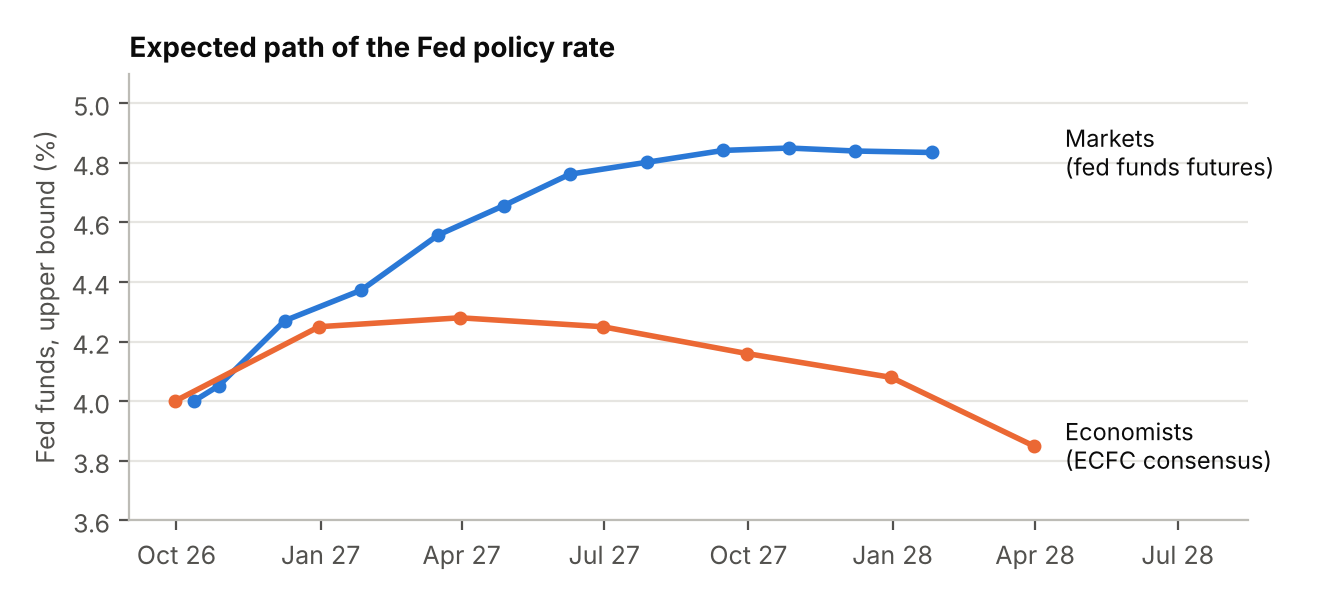
\includegraphics[width=\textwidth]{figures/fed_path}
\caption{Expected path of the Fed policy rate: markets (fed funds futures) vs economists (ECFC consensus)}\label{fig:fedpath}

\smallskip
\footnotesize\emph{Markets: implied upper bound from fed funds futures. \cite{ecfc,wirp}}
\end{figure}

If the economists are right, bonds should rally and growth assets
benefit from lower rates; if the markets are right, inflation remains
sticky and both bonds and equities come under pressure. We read this gap
as the clearest evidence that the next regime is genuinely uncertain,
and it is the starting point of our allocation.

\subsection*{Rates, inflation pricing, credit and the dollar}\label{sec:rates-credit-dollar}

\begin{table}[!htb]
\centering
\small
\caption{Key market indicators}\label{tab:indicators}
\begin{tabular}{@{}lrr@{}}
\toprule
Indicator & 1 year ago & Latest \\
\midrule
US Treasury 1-month yield & 4.20\% & 4.13\% \\
US Treasury 2-year yield & 3.60\% & 4.80\% \\
US Treasury 10-year yield & 4.14\% & 5.24\% \\
US Treasury 30-year yield & 4.72\% & 5.60\% \\
5-year breakeven inflation & -- & 2.34\% \\
10-year real yield (TIPS) & -- & 2.87\% \\
US investment-grade spread (OAS) & 0.75\% & 0.82\% \\
US high-yield spread (OAS) & 2.84\% & 3.15\% \\
VIX & -- & 15.4 \\
EUR/USD, consensus Q3 2026 $\rightarrow$ Q4 2027 & 1.13 & 1.17 \\
\bottomrule
\end{tabular}

\smallskip
\footnotesize\emph{Treasury yields: U.S. Treasury par yield curve \cite{ustreasury}. Breakeven,
real yield, spreads and VIX: FRED (T5YIE, DFII10, BAMLC0A0CM,
BAMLH0A0HYM2, VIXCLS) \cite{fred}. EUR/USD \cite{ecfc}.}
\end{table}

The indicators in Table~\ref{tab:indicators} point to four features of the current market
that shape our universe. The Treasury curve has shifted up by 80--130
basis points from the one-year maturity onwards, so that bonds once
again offer a meaningful income. The inflation priced by the market,
2.34\% over five years, is lower than the consensus forecast of about
2.8\% for the next four quarters, which makes inflation protection
inexpensive. Credit spreads remain tight, so that credit offers little
compensation for its risk, and the consensus expects a mild weakening of
the dollar, which would support non-US assets measured in USD.

\section*{How we built the universe}\label{sec:universe}

\begin{itemize}
\item
  \textbf{No bet on a single regime.} Given the outlook above, we hold
  assets that perform in each of the four regimes rather than picking
  one.
\item
  \textbf{Cheap, broad market exposures.} The policy portfolio drives
  most of the risk and return, and market beta should be bought
  passively. Every ETF tracks a broad market-capitalisation index at low
  cost. Sector, factor and thematic ETFs are left out of the SAA: they
  are bets on expected returns, which we prefer to spend in tactical
  rounds, where they are measured as deviations.
\item
  \textbf{No overlaps.} We did not select ETFs that cover the same
  universe.
\end{itemize}

The result is eight strategic ETFs --- three equity, three fixed income,
two real assets --- plus one T-bill ETF used only as a risk-management
tool.

\section*{The ETFs and why we chose them}\label{sec:etfs}

\subsection*{Equity}\label{sec:equity}

Equity carries the equity risk premium, the most reliable source of
long-run excess return. Instead of a single world ETF we hold three
regional blocks: this gives us control over the regional mix and makes
our outlook visible in the portfolio.

\textbf{VTI --- Vanguard Total Stock Market ETF}

\emph{US equity \textperiodcentered{} CRSP US Total Market Index \textperiodcentered{} listed May 2001 \textperiodcentered{} 3,531
holdings, expense ratio 0.03\% (30 Jun 2026) \cite{vanguardvti}}

\textbf{Why we chose it.} The US is the deepest and most innovative
equity market: it represents 64\% of the MSCI ACWI \cite{msciacwi}. US companies
have delivered the strongest earnings growth of the last decade, driven
by technology and, more recently, the investment cycle in artificial
intelligence, visible in the strength of private investment. US equity
is therefore the main source of expected return in our portfolio.

\textbf{Why VTI and not SPY or VOO.} SPY and VOO hold the 500 largest
companies; VTI holds about 3,500, adding mid and small caps that are
more sensitive to domestic growth and to falling rates, and slightly
less concentrated in the largest technology names.

\textbf{Risks we accept.} High valuations and concentration in mega
caps; with the 10-year yield at 5.24\% bonds are a serious alternative,
which compresses the equity risk premium. We limit these risks with the
concentration cap and by holding equity outside the US.

\textbf{VEA --- Vanguard FTSE Developed Markets ETF}

\emph{Developed ex-US equity \textperiodcentered{} FTSE Developed All Cap ex US Index \textperiodcentered{}
listed July 2007}

\textbf{Why we chose it.} We do not want the portfolio to depend on one
economy. Developed ex-US markets (Europe, Japan, UK, Canada, Australia,
South Korea) trade at a valuation discount to the US and have a
different sector mix --- more financials, industrials and healthcare,
less technology --- so they respond differently to the same shocks. The
fund is unhedged: the expected weakening of the dollar (EUR/USD +3.5\%
to end-2027) would add to its returns in USD.

\textbf{Why VEA and not EFA or VXUS.} EFA excludes Canada and small
caps; VEA includes both. We preferred VEA to an all-in-one ex-US fund
such as VXUS to size emerging markets separately.

\textbf{Risks we accept.} With European growth expected at only
1.3--1.6\%, the case for this position rests on valuations rather than
on earnings momentum, and it may take time to pay off. Many European and
Japanese companies are large exporters, which leaves them exposed to
tariffs and trade tensions, and since the fund is unhedged, a stronger
dollar would reduce its value in USD.

\textbf{IEMG --- iShares Core MSCI Emerging Markets ETF}

\emph{Emerging markets equity \textperiodcentered{} MSCI Emerging Markets Investable Market
Index \textperiodcentered{} listed October 2012}

\textbf{Why we chose it.} Emerging markets offer the best macro
combination of the three regions: growth rising from 3.9\% to 4.4\% in
2027, inflation falling and central banks easing by about 140 bp
\cite{ecfc}, with current-account surpluses of about 3\% of GDP that reduce
their dependence on foreign capital. They also offer lower valuations
and access to the semiconductor supply chain (Taiwan, Korea). A separate
position lets us hold them at least at market weight.

\textbf{Why IEMG and not EEM.} IEMG includes small caps (IMI index) and
is cheaper.

\textbf{Risks we accept.} Emerging markets are more volatile than
developed ones and carry political and regulatory risk, especially in
China, where government intervention can change the outlook for entire
sectors. They also tend to suffer when the dollar strengthens and US
rates rise, as capital flows back to the United States. Finally, the
position partly overlaps with VEA: South Korea is classified as
Developed by FTSE since 2009 \cite{ftsekorea} but remained Emerging for MSCI in
June 2026 \cite{koreatimes}, so it is held in both funds.

\subsection*{Fixed income}\label{sec:fixed-income}

Bonds lower the volatility of the portfolio, which is necessary to stay
within the 7--9\% risk budget, and protect it in a recession with
falling inflation. We hold three different sources of fixed-income
return: US nominal rates, non-US rates and US real rates.

\textbf{BND --- Vanguard Total Bond Market ETF}

\emph{US investment-grade bonds \textperiodcentered{} Bloomberg US Aggregate Float Adjusted
Index \textperiodcentered{} listed April 2007}

\textbf{Why we chose it.} BND holds the US investment-grade market:
Treasuries, agency mortgage-backed securities and IG corporate bonds,
with an intermediate duration. With the 10-year yield at 5.24\% and the
2-year at 4.80\%, bonds pay a meaningful income; economists expect the
10-year yield to fall to about 4.6\% by end-2027 \cite{ecfc}, which would
add a capital gain. Above all, BND is our insurance against a recession:
when growth and inflation fall, central banks cut and bond prices rise.

\textbf{Why intermediate duration, and not TLT.} The US budget deficit
is expected at about 6.5\% of GDP and public debt at 105\% of GDP
\cite{ecfc}: a persistent supply of Treasuries may keep long-term yields
high. Intermediate duration captures most of the recession hedge with
much less of this risk. We excluded high-yield bonds: with a spread of
3.15\% they pay little for a credit risk that rises exactly when
equities fall.

\textbf{Risks we accept.} Since 2021 the stock--bond correlation has
turned positive: when inflation is the problem, bonds and equities can
fall together, as in 2022. Futures also price further Fed hikes.

\textbf{BNDX --- Vanguard Total International Bond ETF}

\emph{International investment-grade bonds, USD-hedged \textperiodcentered{} Bloomberg
Global Aggregate ex-USD Float Adjusted RIC Capped Index (USD hedged) \textperiodcentered{}
listed June 2013}

\textbf{Why we chose it.} Rate cycles outside the US are not
synchronised with the Fed: the ECB rate is about 2.85\% and expected to
ease to 2.5\% by early 2028, and the euro-area 10-year yield is expected
to fall from 3.9\% to 3.7\% \cite{ecfc}. BNDX therefore diversifies the
duration risk of BND. Because it is hedged, it behaves like a bond and
not like a currency position; with US short rates above European and
Japanese rates, the hedge also earns the interest-rate differential.

\textbf{Why BNDX and not IGOV.} IGOV is unhedged: currency moves would
add equity-like volatility to the defensive part of the portfolio.

\textbf{Risks we accept.} A global inflation shock would push yields up
everywhere at once.

\textbf{TIP --- iShares TIPS Bond ETF}

\emph{US inflation-linked Treasuries \textperiodcentered{} listed December 2003}

\textbf{Why we chose it.} Inflation hurts stocks and bonds at the same
time, and 2026 has been a year of rising inflation. TIP is the most
direct protection, and today it is cheap: the 5-year breakeven (2.34\%)
is below the consensus CPI for the next four quarters (2.8\%) and in
line with the consensus for 2028 (2.3\%) \cite{ecfc,fred}. The real yield of
2.87\% means TIP pays a solid return even if inflation simply returns to
target.

\textbf{Why TIP and not STIP.} STIP holds only 0--5 year maturities. We
preferred TIP because, with real yields at their highest in years, we
want to lock in some real-rate duration.

\textbf{Risks we accept.} TIPS protect against inflation, not against
rising real yields: if real rates keep increasing, TIP can lose value
even while inflation is high, as happened in 2022. Conversely, if
inflation falls back faster than the market expects, the inflation
adjustment shrinks and TIP is likely to underperform nominal bonds such
as BND.

\subsection*{Real assets}\label{sec:real-assets}

Real assets protect the portfolio in the two regimes in which equities
and nominal bonds can fall together --- high inflation and supply shocks
--- and are the least correlated part of the universe.

\textbf{GLD --- SPDR Gold Shares}

\emph{Gold \textperiodcentered{} physical gold bullion \textperiodcentered{} listed November 2004}

\textbf{Why we chose it.} Gold has no credit or counterparty risk and
has historically held its value in stagflation, geopolitical crises and
periods of dollar weakness. Official demand has been a structural
support: central banks bought about 850 tonnes in 2025 \cite{wgc}. With an
uncertain outlook, high US public debt and an expected weaker dollar, we
consider gold a necessary insurance.

\textbf{Why GLD and not IAU.} Both hold physical gold; GLD is the
largest and most liquid gold ETF and has the longest history. IAU is
cheaper, but for a position held a few months liquidity matters more
than fees.

\textbf{Risks we accept.} Gold pays no income, and with real yields near
2.9\% the opportunity cost is high. It is volatile and has rallied
strongly: the LBMA price averaged a record USD 4,873/oz in Q1 2026, and
central-bank buying slowed sharply in that quarter (revised to 57
tonnes, with visible selling) \cite{wgc}.

\textbf{BCI --- Bloomberg All Commodity Strategy K-1 Free ETF}

\emph{Broad commodities \textperiodcentered{} Bloomberg Commodity Index Total Return \textperiodcentered{}
listed March 2017}

\textbf{Why we chose it.} Commodities perform best when inflation comes
from supply shocks --- energy disruptions, geopolitical conflicts, bad
harvests --- the scenario in which both stocks and bonds lose, as in
2022. They complement gold: gold reacts to monetary and geopolitical
stress, commodities to the real economy. The total-return index also
earns the T-bill rate on the collateral.

\textbf{Why BCI and not DBC.} BCI follows the Bloomberg Commodity Index:
23 commodities, with no sector above 33\% and no single commodity above
15\% \cite{bcom}. DBC is about half energy and more expensive \cite{teamresearch}.

\textbf{Risks we accept.} Roll costs in markets in contango and sharp
falls in a recession, when demand for raw materials collapses.

\subsection*{Risk-management tool}\label{sec:risk-tool}

\textbf{BIL --- SPDR Bloomberg 1-3 Month T-Bill ETF}

\emph{US Treasury bills, 1--3 months \textperiodcentered{} listed May 2007}

\textbf{Role.} BIL is not a strategic position but a tool to manage the
risk budget. If the eight strategic ETFs together have an ex ante
volatility above 9\%, we scale the risky portfolio down to the 8\%
target and invest the remainder in BIL; if the volatility is already
within the 7--9\% band, BIL is not held at all. Since T-bills barely
move, BIL can only bring the volatility of the portfolio down, never
raise it.

\textbf{Why BIL and not cash.} The Sharpe Ratio is measured on returns
in excess of the 1-month T-bill (4.13\%) \cite{ustreasury}. Cash earns nothing, so
it has an excess return of about \textminus{}4\% a year and lowers the Sharpe
Ratio; BIL earns about the T-bill rate, so its excess return is close to
zero.

\textbf{Why BIL and not SGOV.} SGOV is an equivalent and slightly
cheaper alternative; we use BIL because its longer track record (2007,
against 2020 for SGOV) gives more data if the backtest sample is
extended.
